%%%%%%%%%%%%%%%%%%%%%%%%%%%%%%%%%%%%%%%%%
% fphw Assignment
% LaTeX Template
% Version 1.0 (27/04/2019)
%
% This template originates from:
% https://www.LaTeXTemplates.com
%
% Authors:
% Class by Felipe Portales-Oliva (f.portales.oliva@gmail.com) with template 
% content and modifications by Vel (vel@LaTeXTemplates.com)
%
% Template (this file) License:
% CC BY-NC-SA 3.0 (http://creativecommons.org/licenses/by-nc-sa/3.0/)
%
%%%%%%%%%%%%%%%%%%%%%%%%%%%%%%%%%%%%%%%%%

%----------------------------------------------------------------------------------------
%	PACKAGES AND OTHER DOCUMENT CONFIGURATIONS
%----------------------------------------------------------------------------------------

\documentclass[
  french,
  % twocolumn,
	11pt, % Default font size, values between 10pt-12pt are allowed
	%letterpaper, % Uncomment for US letter paper size
	%spanish, % Uncomment for Spanish
]{fphw}

% \usepackage[fontsize=10.0]{scrextend} % Use this to force the fontsize

%% Commands for numbering paragraphs
\renewcommand\thesection{\Roman{section}}
\renewcommand\thesubsection{\thesection.\arabic{subsection}}
\renewcommand*\thesubsubsection{%
  \Roman{section}.\arabic{subsection}.\alph{subsubsection}%
}

\usepackage{sectsty}
\sectionfont{\sf\bfseries\LARGE\raggedright}

% Template-specific packages
% \usepackage{babel}


% \renewcommand*\familydefault{\sfdefault}
\usepackage[utf8]{inputenc} % Required for inputting international characters
% \usepackage{DejaVuSerifCondensed} 
\usepackage[T1]{fontenc} % Output font encoding for international characters
\usepackage{textcomp}

\usepackage[lf]{venturis}
% \usepackage[libertine]{newtxmath}
\usepackage{libertinust1math}
\usepackage{bm} 

\usepackage{fancyvrb}
\usepackage{fvextra}
\newcommand\userinput[1]{\textbf{#1}}
\newcommand\arguments[1]{\textit{#1}}

\usepackage{amsmath}
\usepackage{mathtools}
\usepackage{xfrac} 
% \usepackage{amssymb}
% \usepackage{enumitem}	%% % To modify the itemize bullet character 

\usepackage{graphicx} % Required for including images
\usepackage[textfont=it,font=small]{caption}  %% To manage long captions in images
\usepackage{subcaption}
\captionsetup{justification=centering}

\usepackage{float}
\graphicspath{ {../img/} }

\usepackage{booktabs} % Required for better horizontal rules in tables

\usepackage{listings} % Required for insertion of code

\usepackage{array} % Required for spacing in tabular environment

\usepackage{enumerate} % To modify the enumerate environment

\newcommand{\tabhead}[1]{{\bfseries#1}}

\usepackage{xcolor}
\usepackage{listings}
\colorlet{mygray}{black!30}
\colorlet{mygreen}{green!60!blue}
\colorlet{mymauve}{red!60!blue}

\usepackage[linkcolor=blue,colorlinks=true]{hyperref}
% \usepackage[colorlinks=true,urlcolor=blue]{hyperref}
\hypersetup{citecolor=blue}

\usepackage{cleveref}
\usepackage{siunitx}

\usepackage[backend=bibtex,style=alphabetic,maxnames=2,natbib=true]{biblatex} % Use the bibtex backend with the alphabetic citation style (compact APA-like)
% \usepackage[backend=bibtex,style=authoryear,maxnames=2,natbib=true]{biblatex} % Use the bibtex backend with the authoryear citation style (which resembles APA)
% \addbibresource{../bib/bibliography.bib} % The filename of the bibliography
\addbibresource{bibliography.bib} % The filename of the bibliography
\usepackage[autostyle=true]{csquotes} % Required to generate language-dependent quotes in the bibliography 
% \renewcommand*{\bibfont}{\tiny} % Pour reduire la taille des references

\usepackage[useregional=numeric]{datetime2}
\usepackage[normalem]{ulem}

% %-------------------------------------------------------------------------------

\newcommand{\myvec}[3]{\begin{pmatrix} #1  \\ #2 \\ #3 \end{pmatrix}}   %% vecteur 3d
\newcommand{\mymat}[9]{\begin{pmatrix} #1 & #2 & #3 \\ #4 & #5 & #6 \\ #7 & #8 &#9 \end{pmatrix}}  %% Matrice 3*3

\renewcommand{\vector}[4]{\begin{pmatrix} #1  \\ #2 \\ #3 \\ #4 \end{pmatrix}}   %% vecteur 4d
% \newcommand{\mymatrix}[16]{\begin{pmatrix} #1 & #2 & #3 & #4 \\ #4 & #6 & #7 & #8 \\ #9 & #10 & #11 & #12 \\ #13 & #14 & #15 & #16 \end{pmatrix}}  %% Matrice 3*3

\newcommand{\hquad}{\hspace{0.5em}} %% Bew command for half quad
\newcommand*\diff{\mathop{}\!\mathrm{d}}
% \setlength\parindent{0pt}	%% To remove all indentations
\newcommand{\bvec}[1]{\bm{\mathrm{#1}}}  %% Use this to make vectors
\newcommand{\bmat}[1]{\bm{\mathsf{#1}}}   %% Use this to make tensors


%----------------------------------------------------------------------------------------
%	ASSIGNMENT INFORMATION
%----------------------------------------------------------------------------------------

\title{\sf\bfseries Compte rendu semaine \#22} % Assignment title
% \title{Difficultés rencontrées} % Assignment title

\author{Roussel Desmond Nzoyem} % Student name 

\date{\DTMdisplaydate{2021}{6}{30}{-1} - \DTMdisplaydate{2021}{7}{05}{-1}} % Due date

\institute{Sorbonne Université \\ Laboratoire Jacques-Louis Lions} % Institute or school name

\class{Stage M2} % Course or class name

\professor{Pr. Stéphane Labbé} % Professor or teacher in charge of the assignment

%----------------------------------------------------------------------------------------

\begin{document}

\maketitle % Output the assignment title, created automatically using the information in the custom commands above

%----------------------------------------------------------------------------------------
%	ASSIGNMENT CONTENT - INTRO
%----------------------------------------------------------------------------------------

Le travail de cette semaine a essentiellement été d'étudier la fracturation des floes de glace. J'ai tout d'abord relu le travail théorique de Dimitri sur le sujet, avant de débuter l'implémentation.

%----------------------------------------------------------------------------------------
% ASSIGNMENT CONTENT - SECTION 1
%----------------------------------------------------------------------------------------

\section*{Tâches effectuées}


\begin{enumerate}
  \item Relecture des chapitres 1 et 2 de la thèse de Dimitri. J'ai aussi lu des parties de la thèse de Mr. Hanen Amor \parencite{amor2008approche}, sous la direction de Mr. Jean-Jacques Marigo. Cette dernière, entièrement consacrée à l'approche variationnelle des lois de Griffith, a aussi considérablement aidé dans la compréhension du problème. 
  \item La deuxième tâche majeure a été l'extraction des déplacements des noeuds de chaque floe impliqués dans la percussion. En effet, il a fallu supprimer le mouvement d'ensemble du floe en comparant les positions des noeuds à celle du centre de masse du floe. Deux graphiques illustratifs sont donnés à la \cref{fig:myfig2}.
  \item La troisième grande tache a été d'étudier la rentabilité d'une fracture suivant le modèle de Griffith. J'ai par exemple marqué sur le dernier graphique de la \cref{fig:myfig2} le moment auquel une fracture apparait sur le floe de gauche (une croix en rouge).  
  \begin{figure}[h]
    \centering
    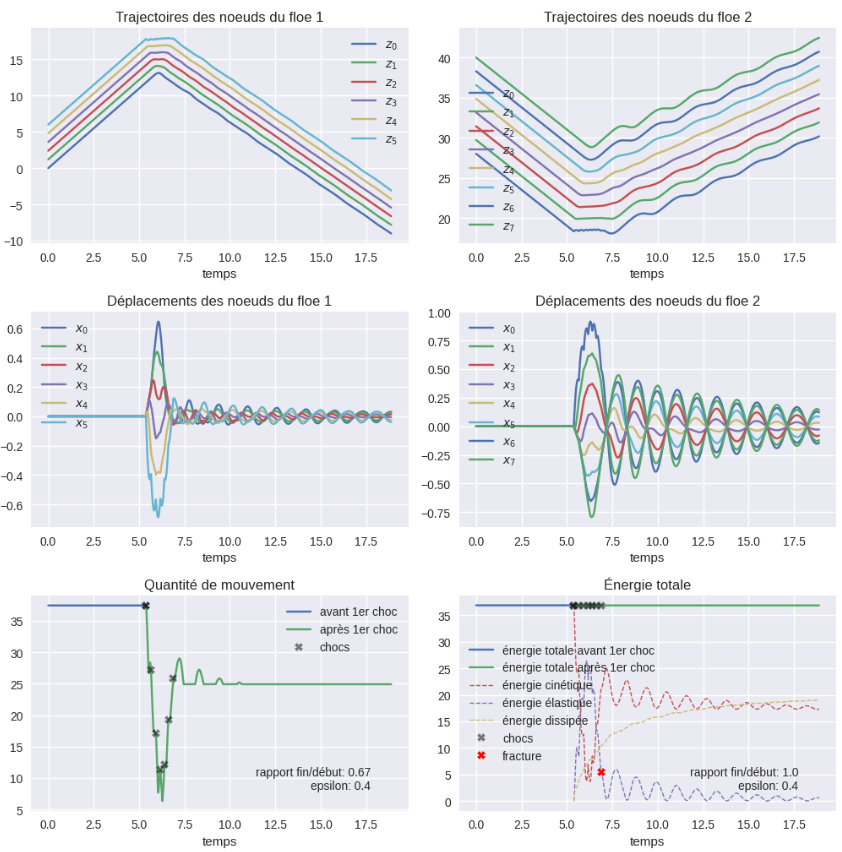
\includegraphics[width=0.80\textwidth]{fracture.png}
    \caption{Différents graphiques pour la simulation 1D. Après la percussion, la fracture illustrée est obtenue sur le floe de gauche pour la rupture de ses deux ressorts les plus à droite. Ici, la ténacité du floe de gauche vaut $0.1$. Il faut noter que plus le matériau est tenace, moins il y a de chance que l'augmentation d'une fracture diminue la somme de l'énergie de déformation et de l'énergie de fracture.}
    \label{fig:myfig2}
  \end{figure}
\end{enumerate}


 
%----------------------------------------------------------------------------------------
% ASSIGNMENT CONTENT - SECTION 2
%----------------------------------------------------------------------------------------

\section*{Difficultés rencontrées}


\begin{enumerate}
  \item La première grosse difficulté est dans la détermination des déplacements de chaque noeud. Je n'ai pas trouvé comment efficacement utiliser le gradient et les vecteurs vitesse pour faire ce travail. À l'inverse, j'ai juste utilisé les positions du centre de masse de l'objet (qui varie au fur et à mesure que le floe se déforme).
  \item La deuxième est que les déplacements ne rentrent pas dans les calculs pour l'instant. En effet, je suis capable de calculer l'énergie de déformation du floe directement à partir de leurs positions. 
  \item Pour l'instant, je considère l'énergie de déformation comme étant juste l'énergie potentielle élastique. J'hésite à définitivement inclure l'énergie dissipée par frottements visqueux.
  \item Le troisième grand problème est : \textbf{qu'es ce qui se passe après la première fracture ?} Tous les déplacements calculés jusqu'a ce niveau deviennent certainement invalides, et je réfléchis sur comment les recalculer de manière efficace.  
  \item Enfin, comment définir exactement la longueur d'une fracture. S'agit-il de la longueur à vide du ressort qui s'est brisé, ou s'agit-il de la longueur du ressort \textbf{au moment} de la fracture. Vu que nous considérons des déplacements élastiques, j'essaie de simplifier cette partie.
\end{enumerate}



%----------------------------------------------------------------------------------------
% ASSIGNMENT CONTENT - SECTION 3
% ----------------------------------------------------------------------------------------
\section*{Travail à venir}

\emph{Par ordre de priorité :}

\begin{enumerate}
  \item Continuation du travail sur la fracture sur le modèle 1D;
  \item Début du même travail sur le modèle 2D;
  \item Mise à jour du rapport de stage.
\end{enumerate}



% %-------------------------------------------------------------------------------
% %							THE BIBLIOGRAPHY
% %-------------------------------------------------------------------------------
\clearpage   % Pour retirer les references de la bare de navigation
\printbibliography


\end{document}
